\section{Wrappers}

As described in Chapter \ref{chapter_dataspaces}, a wrapper is  an interface between the datasource and the dataspace. The wrapper can provide any number of services to access the data of the datasource, but the one service, that every wrapper has to implement, is the keyword search.
In the thesis' project there are three datasources: A SQL database, a pdf file server and a SQL multimedia database serving image files. The SQL database and the multimedia image database contain
structured data while the pdf file server contains semi-structured data.
The following sub sections describe the functionality and implementation of the wrappers for the three datasources in detail.

\subsection{SQL Wrapper}

The task of the SQL Wrapper is to convert the SQL data into rdf and providing a keyword search functionality, as SQL databases doesn't provide such a functionality.

At first we want to look at the conversion from sql to rdf. To do this, the wrapper implements a specialized version of the D2rMap language. D2rMap was designed by Chris Bizer and is  a declarative language to describe mappings between relational databases schemata and OWL/RDFS ontologies\cite{D2rMap_aDatabaseToRdfMappingLanguage}.

D2rMap is a general purpose language to export any sql data to rdf. To better suit the needs for a dataspace wrapper, the language was changed. The changed language is called MeDSpace D2rMap and its language specification can be found in the appendix.

The mapping is done as follows: At first the user specifies mappings in a config file. Each mapping is used to create RDF instances of a certain type. The mapping contains a SQL query, that represents all the data, that is necessary to create the instances. Furthermore, in the mapping are columns specified, that are used to create unique IDs for the created RDF instances.
The next step is to fetch the sql data and to group the record set according to the fore mentioned columns. Now, each row of the grouped record set represents a rdf instance, so the instances can be created. The last step is the creation of the property statements. Important to note is the seperation of the last two steps. Through the seperation it is possible to reference other rdf instances (from the same mapping or another). The mapping process is visualized in figure \ref{D2rMappingProcessFigure}.

\begin{figure}[H]
	\begin{center}
		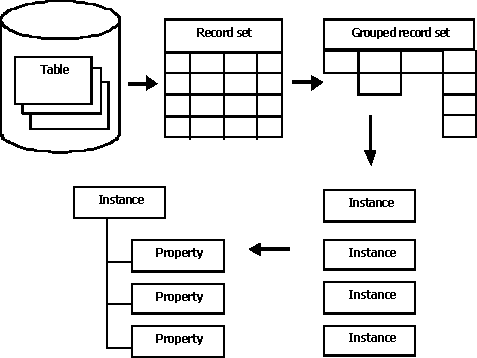
\includegraphics[width=0.75\textwidth]{figures/MappingProcess.pdf}
	\end{center}
	\caption{The D2r mapping process; Taken from \cite{D2rMap_aDatabaseToRdfMappingLanguage}}
	\label{D2rMappingProcessFigure}
\end{figure}

After discussing the SQL to RDF mapping, we look at the keyword search, now:
Mainly there are two possibilities, to implement a keyword search functionality:
\begin{itemize}
	\item {Construct a keyword search query in SQL and let the database answer the query.}
	
	\item {Use a keyword search engine that answers the query based on an external index}
\end{itemize}

At first glance, the first option sounds obviously simple, but after implementing it showed several disadvantages: SQL is not designed to provide search functionality based on keywords. SQL uses the \textbf{\emph{LIKE}} operator for pattern matching. But in order to do a Full-text search, the SQL Query executor cannot use any index resulting in poor query answer performance. Another problem of \emph{LIKE} is, that there is no way to define, that only whole words should be searched and not just sub word matching. Whole word matching is very important, as e.g. a user searching for data about male patients should not also get data about female patients.
As a result, the \emph{LIKE} operator is not suitable for a proper keyword search service as expected to be provided by a dataspace wrapper. Several SQL database vendors provide often own solutions for Full-Text search queries. But these solutions have often other restrictions as e.g. only column fields having the datatype \emph{TEXT} (on MySQL) and the fields have to specified to be fulltext fields, so that the SQL engine is able to create an index for it (at MySQL databases at least).
A Wrapper could use vendor specific services but that would exclude other SQL database vendors, obviously. 

The second option doesn't rise the aforementioned issues of option one. For the Wrapper a keyword searcher was implemented using the fulltext search engine Apache Lucene Core \footnote{\url{https://lucene.apache.org/core/}}. The advantage of using Lucene is it's high-performance and scaling of keyword searches over large data sets. Additionally it allows a fine granular configuration about the query construction and sorts automatically the query result by relevance (so called query result ranking). \\
The major disadvantage of using lucene is that the SQL data have to be extracted and indexed outside the database. If the data changes or rows are added resp. deleted, the index has to be updated accordingly. The update process can be very complex, as not only new data has to be indexed resp. existing data has to be removed, but also data that references the deleted or new data that depends on it.\\
A simpler but obviously slower solution is to reindex the whole data set. Reindexing the whole data set is only advised if updates occur not that often or if it is acceptable if the wrapper updates the index not instantly and thus provides potentially outdated data.

The decision which method is more suitable depends primarily on the use case and the domain. As the project is designed to be used as a test suite for medical datasources and medical science, it is acceptable if the data is outdated to some degree and will be updated not frequently. Changes on the datasource haven't to be updated in near-realtime. Having this in mind, the preferred method for the keyword search functionality clearly is using Apache Lucene Core, as the  advantages clearly outweigh its disadvantages. Thus, a full functional keyword searcher was implemented powered by Lucene.

\subsection{Image Wrapper}
fgfg
\subsection{PDF Wrapper}